\chapter{Low Frequency Radio Astronomy and the Earth's Ionosphere}\label{Ch:Iono}

\textcolor{red}{Draft is still in progress for this chapter, so don't worry about reading it yet.}

Beyond the effects of RFI, the Earth's atmosphere has additional impacts on low frequency radio signals from the universe. These impacts come from interactions between the incoming radio signals and the free electrons in the ionosphere. Impacts include refraction and absorption of radio frequency photons. 

%\begin{figure}[htb]
%\begin{center}
%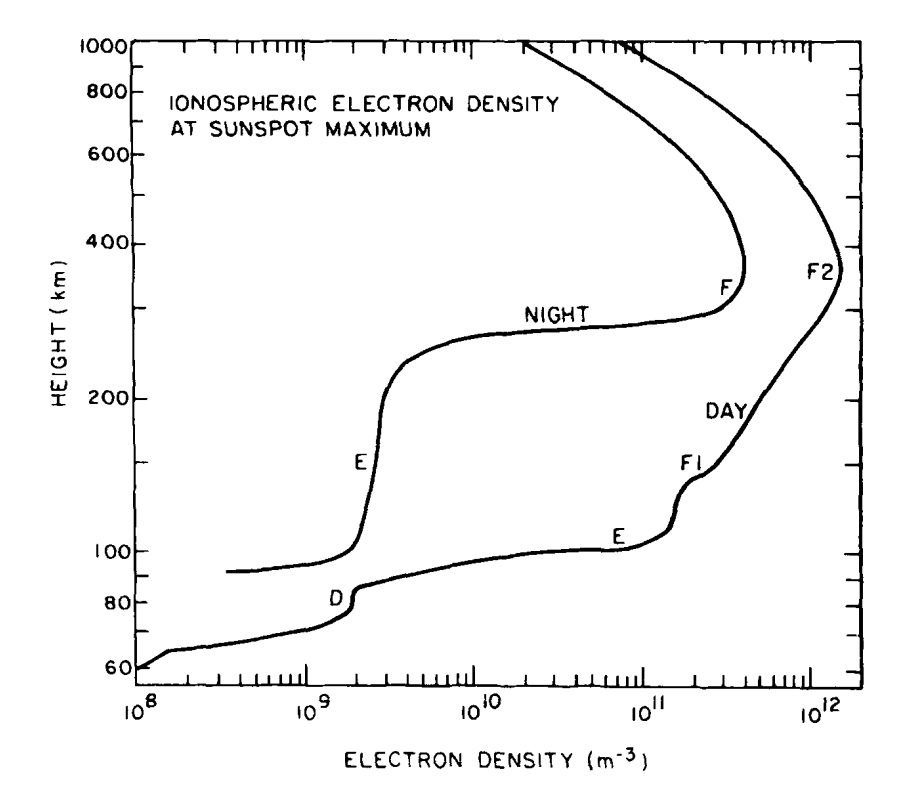
\includegraphics[width=0.95\linewidth]{Ionosphere/figures/atmosphere_layers.jpg}
%\caption{Idealized free electron density distribution in Earth's atmosphere showing the ionosphere's layers during day and night. }
%\label{Fig:atm_layers}
%\end{center}
%\end{figure}

\begin{figure}[htb]
\centering
\begin{minipage}[b]{0.48\textwidth}
\centering
\begin{tabular}{|c|c|}
\hline
Layer & Altitude Range (km) \\
\hline
D & 60-100 \\
\hline
E & 100-150 \\
\hline
F1 & 150-250 \\
\hline
F2 & 250-1000+ \\
\hline
\end{tabular}
\caption{Average distribution of the Earth's ionosphere layers.}
\label{Tab:iono_layer}
\vspace{2cm}
\end{minipage}%
\begin{minipage}[b]{0.02\textwidth}
\hspace{1cm}
\end{minipage}%
\begin{minipage}[b]{0.48\textwidth}
\centering
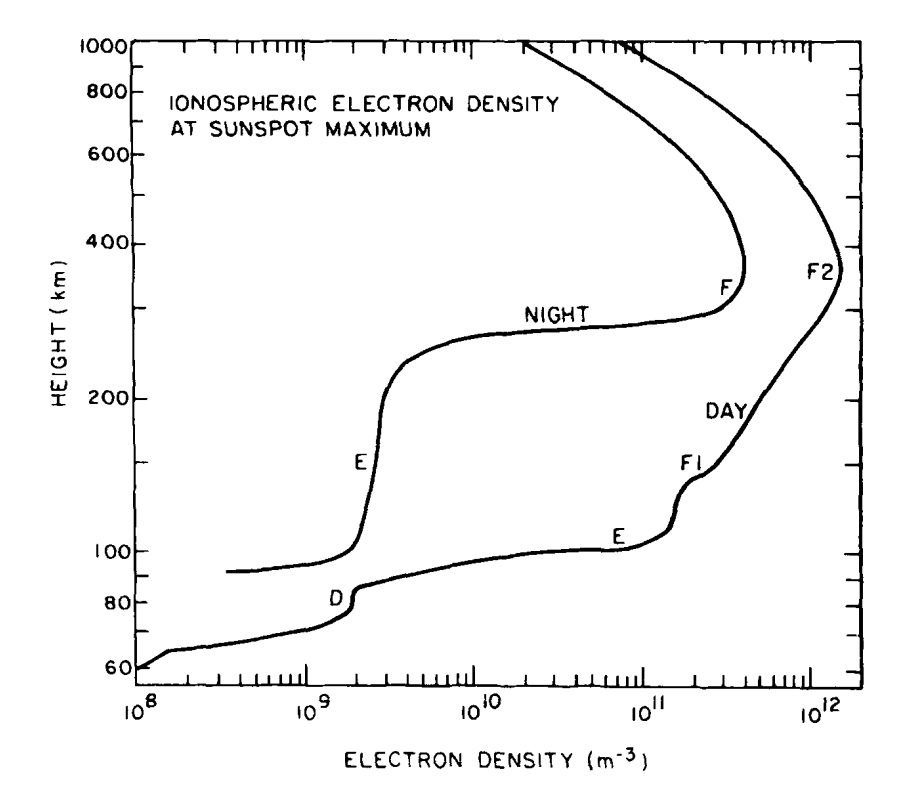
\includegraphics[width=0.95\linewidth]{Ionosphere/figures/atmosphere_layers.jpg}
\caption{Idealized free electron density distribution in Earth's atmosphere showing the ionosphere's layers during day and night. }
\label{Fig:iono_layer}
\end{minipage}
\end{figure}

\section{Earth's Ionosphere}
The ionosphere is located $60 - 1000+$ $km$ above the surface of the Earth and is made up of free electrons and ionized atoms. Neutral atoms in Earth's atmosphere are photoionized by solar radiation, which leads to an altitude dependent distribution of free electrons and ions in the atmosphere.

\subsection{Ionospheric Layers}
This distribution allows us to divide the ionosphere into altitude-dependent regions. The center of each region is defined by a local maximum in the free electrion density distribution as a function of altitude. The regions of the ionosphere are identified in Table \ref{Tab:iono_layer}.  The absolute maximum free electron density ($n_e$) is reached in the F2 layer and is $n_e \cong 10^5 cm^{-3}$ \cite{ionospheres}. 

The presence and width of the ionospheric layers is time dependent and fluctuates over the course of a day. During the day all the layers are present, but during the night some of the layers merge as shown in Figure \ref{Fig:iono_layer}. Electron density distribution also depends on the level of sunspot activity and the specific position (particularly the latitude) on the Earth \cite{thompson_2001}. 

\subsection{Ionosphere Properties}
Free electrons in the ionosphere can be treated like a plasma and will modify the propogation of light. We can quantify it by defining a plasma frequency ($\nu_p$), which has a value equal to:

\begin{equation}
\nu_p = \frac{e}{2 \pi} \sqrt{\frac{n_e}{\varepsilon_0 m}} \cong 9 \sqrt{n_e} Hz
\end{equation}

where $n_e$ is in $m^{-3}$ \cite{thompson_2001}. This plasma frequency changes the index of refraction for the ionosphere compared to free space $n = \sqrt{1-\nu_p^2/\nu^2}$, where $\nu$ is the frequency of the light that is passing through the atmosphere \cite{thompson_2001}. 

\begin{figure}[htb]
\begin{center}
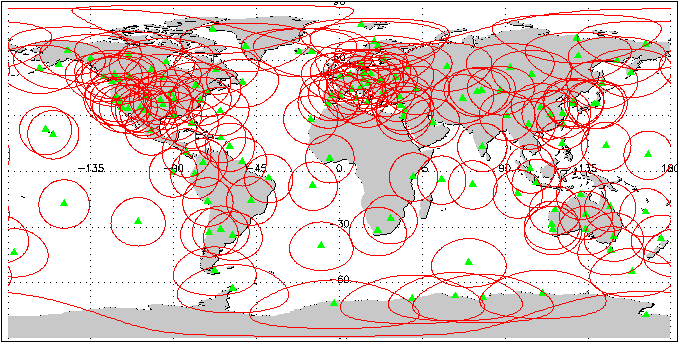
\includegraphics[width=0.95\linewidth]{Ionosphere/figures/gps_sitemap.png}
\caption{Global Map of GPS Network stations used for the quasi-real time maps shown on iono.jpl.nasa.gov}
\label{Fig:gps_stat}
\end{center}
\end{figure}

\begin{figure}[htb]
\centering
\begin{minipage}[b]{0.48\textwidth}
\centering
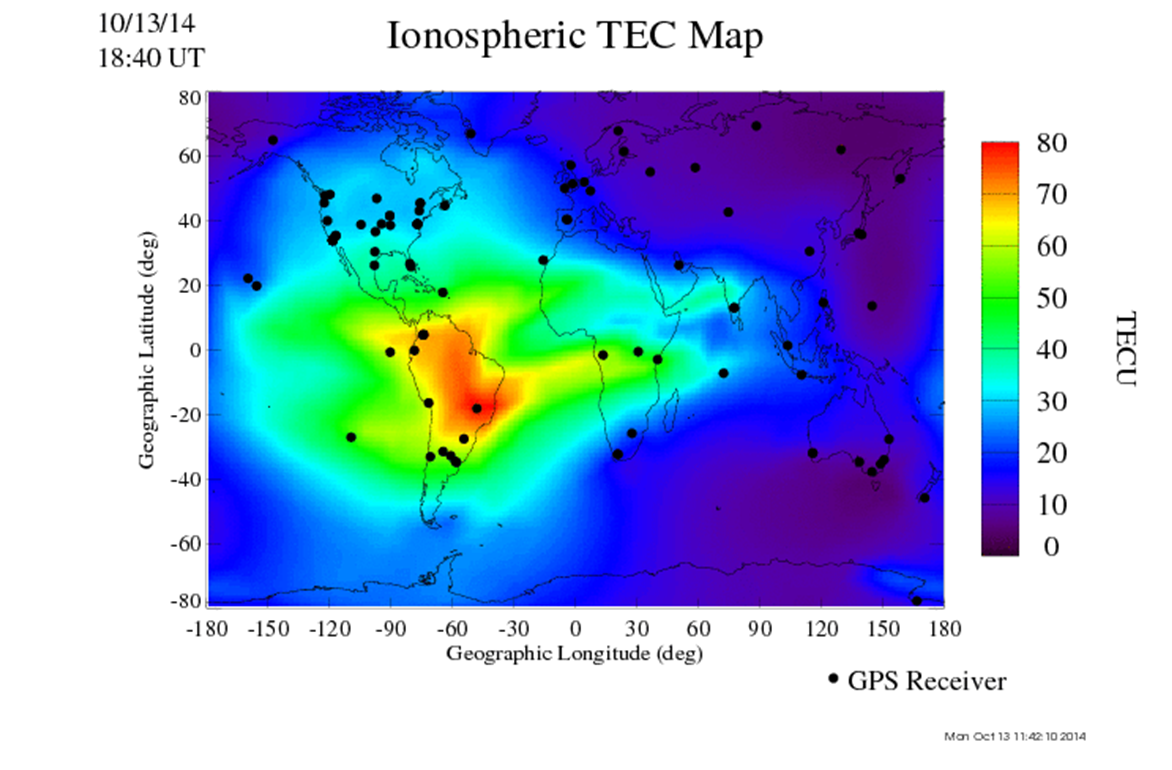
\includegraphics[width=0.95\linewidth]{Ionosphere/figures/TEC_map_20141013_18-40UT.png}
\caption{TEC map from iono.jpl.nasa.gov for October 13th, 2014 at 18:40 UTC.  }
\label{Fig:fall_tec_global}
\end{minipage}%
\begin{minipage}[b]{0.02\textwidth}
\hspace{1cm}
\end{minipage}%
\begin{minipage}[b]{0.48\textwidth}
\centering
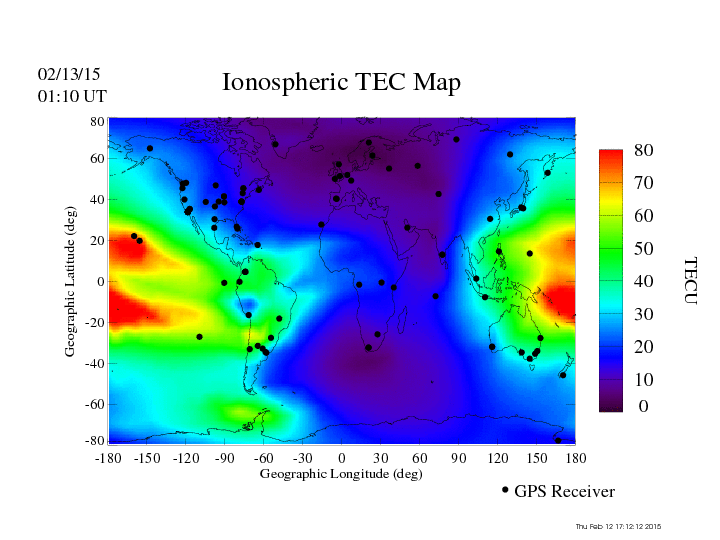
\includegraphics[width=0.95\linewidth]{Ionosphere/figures/TEC_map_20150213_01-10UT.png}
\caption{TEC map from iono.jpl.nasa.gov for February 13th, 2015 at 01:10 UTC.  }
\label{Fig:winter_tec_global}
\end{minipage}
\end{figure}

\section{Total Electron Content}
Measurement of the number of free electrons at a given altitude ($n_e$) can be quite difficult. Instead, scientists typically measure the total electron content (
$TEC$). $TEC$ is the integrated number of free electrons for a skewer through the atmosphere. It is defined as:

\begin{equation}
TEC \simeq -\frac{40.3}{\nu^2} \int_0^\infty n_e (h) dh \simeq -\frac{1}{2} \int_0^\infty  \Big( \frac{\nu_p (h)}{\nu} \Big)^2 dh
\end{equation}

where $h$ is the altitude \cite{thompson_2001}. Total electron content is continually monitored on Earth using measurements from GPS stations around the world. This data is collected by a number of agencies that convert the data into maps. Real time maps of $TEC$ over the entire world made by NASA JPL using the GPS stations shown in Figure \ref{Fig:gps_stat} are available online\footnote{http://iono.jpl.nasa.gov/latest_rti_global.html} and update every 5 minutes. A couple of examples of these maps are Figures \ref{Fig:fall_tec_global} and \ref{Fig:winter_tec_global}, which show the measured $TEC$ distribution for two different times of day (and times of year). The brightest region corresponds to daytime, and areas close to the equator are much brighter than areas near the poles.

\begin{figure}[htb]
\centering
\begin{minipage}[b]{0.48\textwidth}
\centering
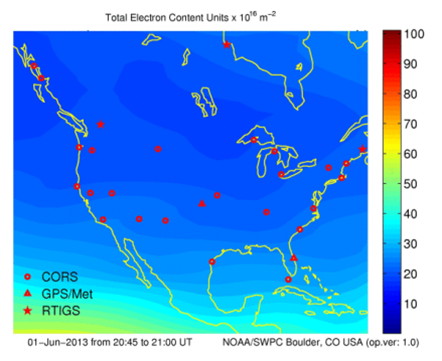
\includegraphics[width=0.95\linewidth]{Ionosphere/figures/NA_TEC_day.png}
\caption{North American TEC map from www.swpc.noaa.gov for June 1st, 2013 at 21:00 UTC.   }
\label{Fig:day_TEC_NA}
\end{minipage}%
\begin{minipage}[b]{0.02\textwidth}
\hspace{1cm}
\end{minipage}%
\begin{minipage}[b]{0.48\textwidth}
\centering
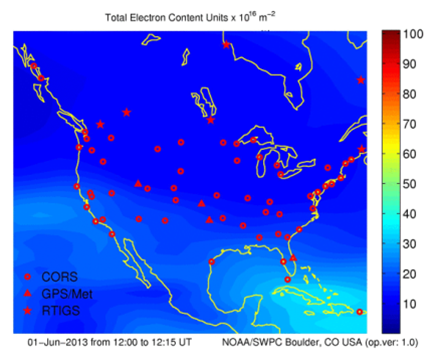
\includegraphics[width=0.95\linewidth]{Ionosphere/figures/NA_TEC_night.png}
\caption{North American TEC map from www.swpc.noaa.gov for June 1st, 2013 at 12:15 UTC.  }
\label{Fig:night_TEC_NA}
\end{minipage}
\end{figure}

In addition, the Space Weather Prediction Center of the National Oceanic and Atmospheric Administration (NOAA) has a model for $TEC$ in North America based on a subset of the GPS stations\footnote{http://www.swpc.noaa.gov/products/us-total-electron-content}. Beyond images, the data is also available online for the most recent few days of data. Using archive data, we can see plots of North American TEC for the Isla Guadalupe deployment in June 2013, as shown in Figures \ref{Fig:day_TEC_NA} and \ref{Fig:night_TEC_NA}. 


\section{Signal variance due to the Ionosphere}
So how does $TEC$ in the ionosphere affect radio signals from the sky? 


\subsection{Refraction}

\subsection{Absorption}


